\section{The Composition of the Income-Poor and Consumption-Poor}\label{sec:composition}

The previous section showed that conclusions about the rate of growth in household resources in the UK, and the evolution of inequality and poverty, are sensitive to the way that resources are measured. None of the analysis made use of the fact that our data tells us about income and consumption for the same households. This section examines how income and consumption can give us different impressions of living standards for a given household.  We focus on the extent to which ``having a low income'' and ``having a low consumption'' identify different households, showing that there are a sizeable number of individuals that are classified as ``poor'' when assessed using household income, but not when assessed using consumption measures (and vice versa). We do this for measures that both do and do not include the implicit income or consumption from housing, and Section \ref{sec:housing} then explores that impact the treatment of that implicit income or consumption from housing has on identifying households that are poor.

\subsection{Rank correlations between income and consumption}

%\subsection{The mismatch between the ``income poor'' and the ``consumption poor''}

Table \ref{table:kendall} shows the similarity of the orderings of households given by our four measures of resources by showing the Kendall rank correlation coefficient, $\tau$, for the selection of years shown in Table \ref{table:prctile}.\footnote{For any two pairs of ranks $(x_{i},y_{i})$ and $(x_{j},y_{j})$ of a variable pair $(x, y)$, define them as concordant if: $(x_{i}-x_{j})(y_{i} - y_{j}) > 0$ and discordant otherwise. Kendall's score is then defined as $\tau = \frac{C-D}{\frac{1}{2}n(n-1)}$, where $C$ is the number of concordant pairs and $D$ is the number of discordant pairs.}

Although there is positive agreement between the rankings (i.e. $\tau>0$ for all pairwise comparisons), all measures give different rankings (i.e. $\tau<1$ for all pairwise comparisons). For the measures that do not include imputed resources from housing, $\tau$ has fallen from 0.49 in 1979 to 0.43 in 2009. Unsurprisingly, $\tau$ for the measures that do include imputed resources from housing is slightly higher (reflecting that both measures contain a identical component equal to the imputed resources from housing); more interestingly, it also shows no clear pattern over time, fluctuating between 0.48 and 0.51.

The values of $\tau$ for pairs of measures that do and do not include the imputed income from housing are, unsurprisingly, much higher, but have also fallen over time, from 0.90 to 0.82 for the two measures of income, and from 0.90 to 0.75 for the two measures of consumption. This reflects a rise over time in the implicit resources from housing that is not perfectly aligned with one's position in the without-housing-resources distribution (and this in turn echoes the finding of Figure \ref{fig:gicall} that the inequality-reducing impact of including resources from housing in a measure of consumption is increasing over time.

\begin{table}[tp!]
\caption{Rank Correlation Between Resource Measures: Kendall's Tau}
\centering
\begin{tabular}{lcccc}
\hline\hline 	
 &  Income IHC & Cons. IHC & Income XHC & Cons. XHC \\
\hline
\multicolumn{5}{l}{\textbf{1979}}  \\
Income IHC &1.0000$^{***}$ & & & \\
 & (0.000)  & & & \\
Cons. IHC & 0.4877$^{***}$&1.0000$^{***}$ & & \\
 & (0.000) &(0.000) & & \\
Income XHC & 0.9006$^{***}$&0.4716$^{***}$ &1.0000$^{***}$ & \\
  & (0.000) &(0.000) & (0.000) & \\
Cons. XHC &0.4733$^{***}$ &0.8980$^{***}$ &0.4890$^{***}$ &1.0000$^{***}$ \\
 & (0.000) &(0.000) & (0.000) & (0.000) \\
\hline
\multicolumn{5}{l}{\textbf{2009}}  \\
Income IHC &1.0000$^{***}$ & & & \\
 & (0.000)  & & & \\
Cons. IHC & 0.4755$^{***}$&1.0000$^{***}$ & & \\
 & (0.000) &(0.000) & & \\
Income XHC & 0.8202$^{***}$&0.3956$^{***}$ &1.0000$^{***}$ & \\
  & (0.000) &(0.000) & (0.000) & \\
Cons. XHC &0.4066$^{***}$ &0.7574$^{***}$ &0.4281$^{***}$ &1.0000$^{***}$ \\
 & (0.000) &(0.000) & (0.000) & (0.000) \\
\hline\hline
\multicolumn{5}{l}{Notes: p-values in brackets. }
\end{tabular}
\label{table:kendall}
\end{table}

\subsection{New title?}

To probe to what extent the different rank correlations are relevant for the low-income population, Figure \ref{fig:overlap} shows trends in the proportion of the population who are in both the bottom decile group of the distribution of income and the distribution of consumption (and calculated separately for measures that do and do not include imputed resources from housing). A perfect rank correlation between a pair of measures would means that this fraction would be 10 percent. However, the average proportion of the population in the bottom decile groups of both of the distributions that do not include imputed income from housing was 2.32\% between 1979 and 2009.\footnote{Although not shown here, the degree of overlap is even lower when one considers all four measures simultaneously: averaged over each year in our data, only 1.69\% of the population was in the bottom decile group of all four resource distributions on average.} For the distributions of the resources that do included imputed resources from housing, this was higher, at 3.96\%, and is on an increasing trend. As before, the fact that the fraction deemed poor on both income and consumption is higher when we include imputed resources from housing than when we do not reflects that the two measures that include imputed resources from housing are (weakly) positively correlated by construction, and the fact that the fraction deemed poor on both is rising over time when using a resource measure that includes imputed resources from housing reflects that the imputed income from housing is growing in importance at the bottom of the resource distribution.


\begin{figure}
\caption{In Bottom Decile of Income and Consumption Distributions}
\centering
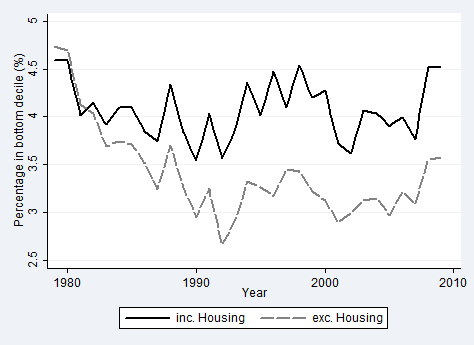
\includegraphics[width=.7\linewidth]{pictures/overlap.png}
\label{fig:overlap}
\end{figure}

\subsection{New title?}
As income and consumption do, then, give different orderings of households and identify different households as having low resources, it is worth assessing which measure better correlates with other indicators of low living standards. We proceed using an approach suggested by \citet{meyer2003measuring}.
We define four groups $BrInc_{low}$. $BrInc_{notlow}$, $Con_{low}$
and $Con_{notlow}$, where the subscript `low' refers to those households
lying in the bottom 10 per cent of the consumption or income distribution,
and `notlow' to those households lying in the upper 90 per cent of
the distribution in question, and BrInc
and Con refer to broad income and consumption respectively. Defining
$X$ as some outcome that (at least arguably) correlates positively
with living standards (for example having health insurance or owning
one's own home), and defining $X(y)$ as the mean outcome for group
$y$, we then calculate a difference-in-difference type measure:

\begin{equation}
\left[X(Con_{low})-X(Con_{notlow})] - [X(BrInc_{low})-X(BrInc_{notlow})\right]\label{eq:diffindiff}
\end{equation}


This will be negative if being in the bottom decile group of reported
consumption is a better indicator of poor outcomes than being in the
bottom decile group of reported income.

We calculate this measure for ownership of various consumer durables
(dishwasher, washing machine, central heating, computer, DVD player,
access to the internet at home, a TV, subscription TV), having health
insurance, owning one or more cars, owning their own house, and the
number of rooms in the house. We noted above that the measure of consumption
used here does not include any spending on durables. This is to avoid
the generation of mechanical (and not particularly informative) relationships
between the measure of consumption and ownership of durables.

The results are shown in Table \ref{tab:Rel_cons_inc_all}. All but
one of the statistics have a negative sign and are statistically significant;
the exception is owning a TV (perhaps unsurprisingly as the vast majority
of all households now own a TV). Although the LCFS provides
a limited number of alternative measures of living standards, overall
we conclude emphatically that having a low recorded consumption is
a better guide to who has a low living standard than having a low
reported income.

% Table generated by Excel2LaTeX from sheet 'Table 6'
\begin{sidewaystable}
%\begin{table}[htbp]
\centering
\caption{The relationship between low consumption, low income and other outcomes, all households}
\begin{tabular}{lcccccccc}
\addlinespace
\toprule
& (1)    & (2)    & (3)    & (4)    & (5)    & (6)    & (7)    & N \\
\midrule
& $X(Inc_{low})$ & $X(Inc_{notlow})$ & (1)-(2) & $X(Con_{low})$ & $X(Con_{notlow})$ & (4)-(5) & (6)-(3) &  \\
Wsh. Mch. & 0.92  & 0.96  & -0.04 & 0.84  & 0.96  & -0.12 & -0.083*** & 52,796 \\
Cent. Heat. & 0.92  & 0.94  & -0.03 & 0.89  & 0.95  & -0.06 & -0.030*** & 52,796 \\
Dishwash. & 0.20   & 0.36  & -0.16 & 0.06  & 0.37  & -0.31 & -0.151*** & 52,796 \\
DVD   & 0.59  & 0.61  & -0.03 & 0.42  & 0.63  & -0.22 & -0.189*** & 52,796 \\
TV    & 0.98  & 0.99  & -0.01 & 0.98  & 0.99  & -0.01 & 0.002 & 52,796 \\
Pay TV & 0.30   & 0.39  & -0.09 & 0.18  & 0.40   & -0.22 & -0.134*** & 52,796 \\
PC    & 0.54  & 0.64  & -0.10  & 0.24  & 0.68  & -0.44 & -0.335*** & 52,796 \\
Internet & 0.41  & 0.56  & -0.15 & 0.15  & 0.59  & -0.44 & -0.286*** & 52,796 \\
Car   & 0.53  & 0.78  & -0.25 & 0.24  & 0.82  & -0.57 & -0.321*** & 52,796 \\
Two cars & 0.14  & 0.33  & -0.19 & 0.02  & 0.34  & -0.32 & -0.130*** & 52,796 \\
Own hse. & 0.37  & 0.74  & -0.38 & 0.32  & 0.75  & -0.43 & -0.055*** & 52,796 \\
No. rooms & 4.97  & 5.38  & -0.41 & 4.5   & 5.44  & -0.94 & -0.528*** & 52,796 \\
Health ins. & 0.05  & 0.13  & -0.08 & 0.02  & 0.13  & -0.12 & -0.036*** & 52,796 \\
\bottomrule
\multicolumn{9}{c}{\parbox[b]{18cm}{
{\footnotesize{Source: Authors' calculation using Expenditure and Food Survey/Living Costs and Food Survey 2001/02- 2009. \\*
Notes: Column (7) gives the quantity expressed in equation (3). Negative numbers indicate that consumption is better correlated with the outcome in the left-hand column (e.g. having a washing machine, owning one's own home) than is income. Other columns give the individual components of the quantity in equation (3). *** indicates significant at the 1\% level, ** indicates significant at the 5\% level, * indicates significant at the 10\% level. Confidence intervals are calculated by bootstrapping with 999 replications.}}}}
\end{tabular}%
\label{tab:Rel_cons_inc_all}%
%\end{table}%
\end{sidewaystable}%


\subsection{New title?}
%Given the differences in ranking between resource distributions, there are a number of individuals for whom resource distribution matters for whether they are identified as having low living standards: they would be classed as living in poverty if their living standards were measured using income but not if they were measured by consumption and vice versa. It is informative to dig deeper into differences in the characteristics of the individuals who make up the bottom deciles of the different resource distributions.

%We begin with a simple descriptive analysis.
We now examine the composition of the bottom of each of the income and consumption distribution. Indeed, analysis such as this is extremely relevant for those interested in designing policies targeted at those with a low living standard.

We begin with a relatively simple breakdown, asking to what extent individuals with the lowest resources are the elderly, or are children. Figure \ref{fig:age_comp} shows, in each year and for each of our four measures of household resources, the proportion of the bottom decile group who are working-age adults (panel (a)) and the elderly [Mike asks Abi: how define ``pensioners'' or the ``elderly''?] (panel (b)), with children representing the omitted category [Mike asks Abi: please can we show the graph for children?].

There is a consistent story across all measures that the proportion of the bottom decile group who are pensioners is considerably lower in 2009 than it was in 1979. [LINK TO OTHER WORK.] But the extent to which the group deemed to have low resources contains the elderly depends on how resources are measured. Two facts are clear. First, regardless of the treatment of resources from housing, the proportion of the bottom decile group who are pensioners is lower when assessed using income than when using consumption.\footnote{Crossley and O'Dea (2010) present an analysis that is consistent with this finding by showing the median saving rate (defined as \emph{income less spending} as a fraction of \emph{income} by age that is implied by the same LCFS data as we analyse here. These implied saving rates rise strongly with age for those aged over 60; equivalently, many elderly households report in the LCFS cash spending levels that are considerably lower than their cash income. This seems counter-intuitive, at least if one has in mind a simple lifecycle model of asset accumulation and decumulation. Finch and Kemp (2006), analysing the same data that we use, concluded that ``although the evidence has been far from conclusive, low spending amongst pensioner households appears to reflect an inter-related set of factors associated with increasing frailty and declining mobility, leading to reducing social participation and contracting social networks.'' Put more crudely, they found no evidence that the data was under-recording spending, and attributed the low levels of spending to a declining ability (or need) to spend money as older people's health deteriorated. Using qualitative research, Dominy and Kempson (2006) found considerable evidence of saving going on amongst the elderly, much of which would probably be considered by economists as precautionary saving for unexpected, lumpy items of spending. In the absence of high-quality longitudinal data on household wealth, more research is needed before we can conclude whether the LCFS is offering a correct impression of the savings behaviour of the elderly, and if so, what economic explanation lies behind it. Until, we need to be mindful that income and consumption do give differing impressions of the living standards of the elderly in ways which may be different from conventionally assumed. We will return to this discussion in Section \ref{sec:housing}.[Mike notes: yes I know it's a big footnote. Abi has this material in the text later on, but I think a mention of it needs to come here. Or do we need to put this in the main text and make more of it?]}

Second, moving to a measures of resources that includes imputed resources from housing reduces the proportion of the bottom decile group who are pensioners (particularly when using consumption). In the first two cases, the opposite is true for the  proportion who are working-age adults, for the last case, the same is also true for the proportion who are working-age adults, implying that moving to a measures of resources that includes imputed resources from housing increases the proportion of the bottom decile group who are children.

\begin{figure}
\caption{Age Composition of Bottom Decile Group of Income and Consumption}
\centering
	\subfloat[Working age]
	{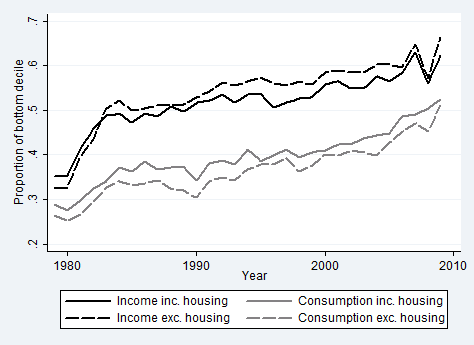
\includegraphics[width=.5\linewidth]{pictures/dec_comp2.png}} \\
	\subfloat[Pensioners]
	{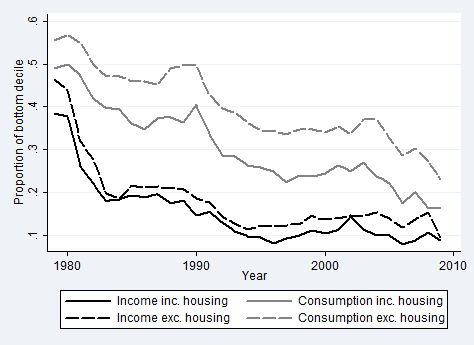
\includegraphics[width=.5\linewidth]{pictures/dec_comp3.png}} \\
	\subfloat[Children]
	{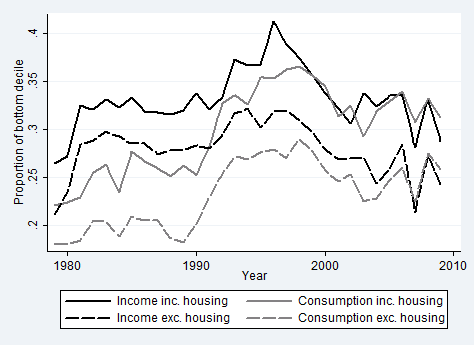
\includegraphics[width=.5\linewidth]{pictures/dec_comp1.png}} \\
\label{fig:age_comp}
\end{figure}

Figure \ref{fig:pov_comp} shows the proportion of the bottom decile group with low levels of educational qualifications (defined as leaving school at, or younger than, 16 years old). The most striking finding is the stark change over time whereby the bottom decile group (however measured) has become increasingly well educated. However, what is more interesting is that those with a low consumption are more likely to be low educated compared to those with a low income. Because we would expect levels of education to be strongly correlated with levels of resources (including those coming from housing) assessed over a lifetime, then this suggests that identifying the poor using low consumption is better at identifying those more likely to be long-term poor than using income, as does using a measure that includes the imputed resources from housing.

\begin{figure}
\caption{Proportion of More Educated Individuals in Bottom Decile Group of Income and Consumption}
\centering
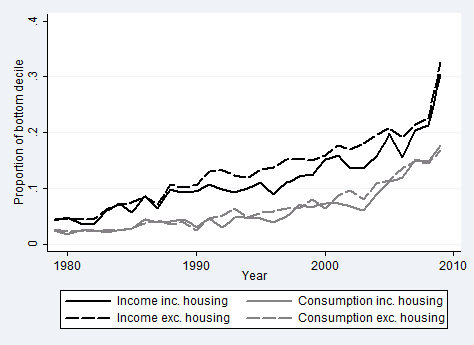
\includegraphics[width=.7\linewidth]{pictures/dec_comp4.png}
\label{fig:pov_comp}
\end{figure}

We now probe this suggestion further by testing the significance of observed demographic factors as predictors of having a low living standard assessed using both income and consumption. To do this, we estimate a multinomial logit model with four outcome categories: (1) in the bottom decile group of both income and consumption resource distributions; (2) in the bottom decile group of the income distribution but not the consumption distribution; (3) in the bottom decile group of the consumption distribution but not the income distribution; (4) not in the bottom decile group of either the income and consumption distributions. With ``not in the bottom decile group of either the income and consumption distributions'' as the reference category, we then test for equality of the relative risk ratios that correspond to a given demographic characteristic.\footnote{An alternative approach would be to estimate separate logits for being in the bottom decile group of income and of consumption, and comparing coefficients across models. However, as noted in Allison (1999), coefficients in binary regression are confounded with residual variation, and so differences in the amount of residual variation between groups can produce differences in slope coefficients between groups that are not indicative of causal differences. Although solutions have been proposed to deal with this problem, all have their drawbacks (see, for example, Williams (2009) and Mood (2010)) and there is yet no consensus. We therefore we estimate a multinomial logit model and test for significant differences in the impact that characteristics have in predicting income-only-poverty versus consumption-only-poverty. If a characteristic was just as effective at predicting income-poverty as it was consumption-poverty - which is the interpretation that people like to make when logit coefficients are found to be equal to each other - then these relative risk ratios in our multinomial logit should not be significantly different from each other.}

The results are in Table \ref{table:multinom_incon}, which shows the relative risk ratios of several demographic characteristics for the outcomes ``in the bottom decile group of both income and consumption resource distributions'', $r_{IC}$, ``in the bottom decile group of the income distribution but not the consumption distribution'', $r_{I}$, and ``in the bottom decile group of the consumption distribution but not the income distribution'', $r_{C}$.  The key parameter of interest, reported in the column titled $r_{I}-r_{C}$, is then the difference between the relative risk ratio of being ``in the bottom decile group of the income distribution but not the consumption distribution'' and ``in the bottom decile group of the consumption distribution but not the income distribution'', and we report the $\chi^{2}$ test statistic for their equality. Note that a negative (positive) value in the $r_{I}-r_{C}$ column means that that demographic characteristic is a better predictor of having a low consumption than it is for having a low-income. \footnote{The results given here are for the sub-period 1999-2009. The results for earlier decades show the same qualitative story, and can be found in the Appendix \ref{sec:annex_results}.}

To give an illustration of how to interpret this, recall that Figure \ref{fig:pov_comp} showed that the bottom decile group of the consumption distribution contained more low-educated individuals than the bottom decile group of the income distribution, meaning that having a low education is a better predictor of having a low consumption than it is of having a low income. This is reflected in the left-hand panel of Table \ref{table:multinom_incon}, where there is a higher relative risk ratio on ``left school $\leq16$'' in column $r_{C}$ (2.460) than there is in column $r_{I}$ (1.300). The fourth column of the left-hand panel, $r_{I}-r_{C}$, reports the difference in these relative risk ratios, confirming that it is negative, and statistically different from zero at the 5\% level. The interpretation is, therefore, that  having a low education is more strongly correlated with having a low consumption than having a low income.

Looking at all rows of Table \ref{table:multinom_incon}, the left-hand panel shows that the risk of being in the bottom decile group of the income distribution but not of the consumption distribution is higher for those who are under 30, highly educated, and unemployed, and, conversely, the risk of being in the bottom decile group of the consumption distribution but not of the income distribution is higher for those who over 60, have low education, and who are not unemployed.  Finally, the left-hand panel of the table repeats the analysis but using measures of income and consumption that do not add resources from housing. The conclusions are very similar: the risk of being in the bottom decile group of the income distribution but not of the consumption distribution where we do not add resources from housing is higher for those who under 30, highly educated, and unemployed.

\begin{sidewaystable}
\caption{Demographics and the Bottom Decile, 1999-2009: Multinomial Logit Relative Risk Ratio [Mike asks Abi and Cormac: can you provide a more informative or descriptive title]}
\centering
\begin{tabular}{l|cccc|cccc}
\hline\hline
	& \multicolumn{4}{c}{\textbf{IHC Bottom Decile}} &  \multicolumn{4}{c}{\textbf{XHC Bottom Decile}} \\
	&	Inc \& Cons.	&	Inc. Only	&	Cons. Only	&	Diff.	&	Inc \& Cons	&	Inc Only	&	Cons. Only	&	Diff. 	\\
	&	$r_{IC}$	&	$r_{I}$	&	$r_{C}$ &	$r_{I}$-$r_{C}$&	$r_{IC}$	&	$r_{I}$	&	$r_{C}$	&	$r_{I}$-$r_{C}$\\
 & se & se & se & $\chi^{2}$  & se & se & se & $\chi^{2}$ \\
\hline
Left school $\leq$ 16	&	       2.370***	&	       1.20***	&	       2.68***	&	-1.48***	&	     					  1.47*** 	&	1.07	&	       2.21***	&	-1.14***	\\
                    	&	       0.252   	&	0.09	&	0.28	&	58	
		&	       0.088   	&	0.06	&	0.15	&	55	\\
Left school $>$ 19	&	       1.71***   	&	       0.92  	&	       0.99* 	&	-0.07	&
				       0.85*   	&	0.94	&	0.96	&	-0.02	\\
                    	&	       0.177   	&	0.07	&	0.11	&	0.25	&	
			      0.069   	&	0.09	&	0.07	&	0.05	\\
Age $<$ 30	&	       1.150   	&	       1.55***	&	1.32***	&	0.23***	&
			       1.21*   	&	       1.36***	&	1.25***	&	0.10	\\
                    	&	       0.142   	&	0.11	&	0.12	&	4.51	&	
			       0.133   	&	0.08	&	0.10	&	1.9	\\
Age 30-40	&	       1.032   	&	1.14**	&	       1.11** 	&	0.03	&	
			       0.85***	&	1.02	&	1.09***	&	-0.07	\\
                    	&	       0.068   	&	0.07	&	0.05	&	0.12	&	
			       0.047   	&	0.05	&	0.05	&	0.64	\\
Age 50-60	&	       0.791**  	&	       0.85*** 	&	0.96	&	-0.11	&
			       0.91   	&	       0.82***  	&	1.02	&	-0.20***	\\
                    	&	       0.093   	&	0.04	&	0.03	&	3.22	&	
			       0.055  	&	0.04	&	0.06	&	7.00	\\
Age 60-70	&	       0.263***	&	       0.41***	&	       1.00 	&	-0.59***	&	       						0.14***	&	       0.36***	&	1.10	&	-0.74***	\\
                    	&	       0.034   	&	0.04	&	0.08	&	46.51	&	
			    0.012   	&	0.03	&	0.07	&	113	\\
Age $\geq$ 70	&	       0.331***	&	       0.20***	&	       2.12***	&	-1.92***	&	       					0.20***	&	       0.21***	&	       2.46***	&	-2.25***	\\
                    	&	       0.051   	&	0.02	&	0.18	&	284	&	       0.03   	&	0.01	&	0.24	&	445	\\
Workless	&	       13.130***	&	       6.57***	&	       3.17***	&	3.41***	&	       						17.2***	&	       7.54***	&	       3.54***	&	4.00***	\\
	&	1.33	&	0.52	&	0.26	&	42	&	
	1.43	&	0.38	&	0.18	& 	82 \\
Self Employed	&	       13.130***	&	       3.88***	&	       0.92 &	2.96***	&	       							1.64***	&	       4.23***	&	       0.89 &	3.34***	\\
	&	1.33	&	0.35	&	0.08	&	88	&
		0.20	&	0.37	&	0.09		& 121	\\
Couple	&	      0.776***	&	       0.85***	&	      0.72***	&	0.13**	&	       						0.96	&	      1.11	&	      0.93	&	0.19**	\\
			&	0.069	&	0.08	&	0.05	&	5.5	&
			0.07	&	0.10	&	0.06		&4.3	\\
Single	&	     0.993	&	       1.14	&	      0.90	&	0.24**	&
		       3.43***	&	       2.22***	&	       2.42***	&	-0.21	\\
	&	0.101	&	0.12	&	0.07	&	6.5	&
		0.280	&	0.19	&	0.17		& 0.9	\\
Children	&	      2.707***	&	       1.53***	&	       2.63***	&	-1.10***	&	       					0.85***	&	       1.12	&	       1.81***	&	-0.69***	\\
	&	0.234	&	0.12	&	0.09	&	124	&	
		0.066	&	0.08	&	0.06		& 55	\\
Constant            	&	       0.013***	&	       0.056***	&	       0.085***	&		&	      					 0.02***	&	       0.069***	&	       0.074***	&		\\
                    	&	       0.00   	&	0.01	&	0.01	&		
		&	       0.00   	&	0.01	&	0.01	&		\\
\hline\hline
\multicolumn{9}{l}{Significantly different from zero at the  10\% ($\star$), 5\% ($\star\star$) and 1\% level ($\star\star\star$).} \\
\multicolumn{9}{l}{Omitted variables: Left school between 17-18 years old, household head aged between 40 and 50 years, employed. }
\end{tabular}
\label{table:multinom_incon}
\end{sidewaystable}


%\subsection{Need title?}

Overall, the results reported in Table \ref{table:multinom_incon} provides further weight for our hypothesis that those found at the bottom of the income distribution are those who are more likely to be temporarily poor - the young, those with high levels of education, and the unemployed (who will presumably soon become employed - than those found at the bottom of the income distribution. [Mike says: although I note that there is an issue with age, and the non-spending older people. REFER BACK TO EARLIER DISCUSSION].

We explore this further in Table \ref{table:interact}, which now interacts age, education and unemployment. Focusing on the  $r_{I}-r_{C}$ column in the left-hand panel, the results show that those characteristics that are more associated with being consumption-poor than income-poor are: having a low education, and being aged over 60. Being out of work is more associated with being income-poor than being consumption-poor, and especially so for those aged under 30, but this effect is reduced for those who are both low-education and unemployed, or aged over 60 and unemployed. As above, if we think of those who are young and out-of-work as more likely to be in a position of temporary low income than those who are older and out-of-work, and similarly for those with high levels of education compared to those with low levels of education, then having a low consumption seems more likely to identify those individuals who are at greater risk of long-term poverty.\footnote{Results in the right-hand panel are qualitatively identical.}


\begin{sidewaystable}
\caption{Age, Education \& Unemployment, 2000-2009: Multinomial Logit Relative Risk Ratio}
\centering
\begin{tabular}{l|cccc|cccc}
\hline\hline
	& \multicolumn{4}{c}{\textbf{IHC Bottom Decile}} &  \multicolumn{4}{c}{\textbf{XHC Bottom Decile}} \\
	&	Inc \& Cons.	&	Inc Only	&	Cons. Only	&	Diff.	&	Inc \& Cons	&	Inc Only	&	Cons. Only	&	Diff. 	\\
	&	$r_{IC}$	&	$r_{I}$	&	$r_{C}$ &	$r_{I}$-$r_{C}$&	$r_{IC}$	&	$r_{I}$	&	$r_{C}$	&	$r_{I}$-$r_{C}$\\
 & se & se & se & $\chi^{2}$  & se & se & se & $\chi^{2}$ \\
\hline
Left school $\leq$ 16	&	       2.63***	&	       1.32***	&	       2.25***	&	-0.92***	&	       						1.20   	&	       1.20***  	&	      1.96***	&	-0.75***	\\
                    				&	       0.43   	&	0.09	&	0.21	&	21	&	
			      				 0.18   	&	0.08	&	0.17	&	20	\\
Left school $>$ 19	&	       1.13   	&	       0.71***	&	       0.81*** 	&	-0.10	&	       						0.62**   	&	       0.82** 	&	0.93	&	-0.12	\\
                   	 	&	       0.23   	&	0.06	&	0.10	&	0.80	&	
			  	   0.12   	&	0.06	&	0.10	&	1.00	\\
Workless*Left school $\leq$ 16	&	       0.90   	&	0.86	&	       1.39**  	&	-0.53***	&	       					1.27  	&	       0.82**  	&	1.021	&	-0.39***	\\
                    	&	       0.17   	&	0.09	&	0.19	&	8.7	&
	       0.22   	&	0.08	&	0.14	&	7.4	\\
Workless*Left school $>$ 19	&	       2.10***   	&	       1.96***	&	1.48**	&	0.49	&	       1.63 **  	&	       1.39***	&	1.01	&	0.38***	\\
	&	       0.50   	&	0.25	&	0.28	&	1.7	&
	       0.37   	&	0.17	&	0.16	&	3.0	\\
Age $<$ 30	&	       1.30*  	&	       1.62*** 	&	1.35***	&	0.27	&	
			       1.07   	&	1.25***	&	1.27**	&	-0.02	\\
	&	       0.20   	&	0.15	&	0.14	&	1.8	&	
			    0.19  	&	0.11	&	0.13	&	0.01	\\
Age 30-40	&	       0.85   	&	1.11	&	       1.132 	&	-0.02	&	
			       0.78  	&	      0.97  	&	1.08	&	-0.11	\\
                    	&	       0.11  	&	0.08	&	0.09	&	0.03	&	
			       0.13   	&	0.06	&	0.09	&	1.12	\\
Age 50-60	&	       0.70**  	&	0.84**	&	0.82**	&	0.02	&	
			       0.95   	&	       0.81***  	&	0.99	&	-0.18	\\
                    	&	       0.12  	&	0.07	&	0.08	&	0.04	&	
			       0.16   	&	0.06	&	0.10	&	2.7	\\
Age 60-70	&	       0.47** 	&	0.72***	&	       1.245**	&	-0.52***	
		&	       0.42*** 	&	       0.62***	&	1.28	&	-0.66***	\\
                    	&	       0.14   	&	0.09	&	0.17	&	5.32	&	
			       0.13   	&	0.07	&	0.16	&	20	\\
Age $\geq$ 70	&	       0.34***	&	       0.18***	&	       1.99***	&	-1.81***	&	       						0.21***	&	       0.21***	&	       2.29***	&	-2.08***	\\
                    	&	       0.03   	&	0.02	&	0.17	&	452	&	
			      0.02   	&	0.02	&	0.18	&	573	\\
Workless*Age $<$ 30	&	       0.87   	&	0.82	&	0.84	&	-0.102
				&	       1.23   	&	1.16	&	0.91	&	0.25	\\
				&	       0.16  	&	0.11	&	0.13	&	0.03	&	
					   0.25   	&	0.15	&	0.14	&	2.0	\\
Workless*Age 30-40	&	       1.30*   	&	1.03	&	0.93	&	0.10	&	
				       1.11   	&	1.14	&	0.97	&	0.17	\\
			&	       0.20   	&	0.12	&	0.12	&	0.44	&	
				      0.20   	&	0.12	&	0.12	&	1.3	\\
Workless*Age 50-60	&	       1.15  	&	0.95	&	1.28	&	-0.32	&	
				       0.93   	&	0.97	&	1.01	&	-0.04	\\
			&	       0.22   	&	0.11	&	0.18	&	2.9	&	
				   0.17   	&	0.10	&	0.13	&	0.1	\\
Workless*Age 60	&	       0.52**   	&	       0.47***	&	       0.73**  	&	-0.26**	&	
			   0.31***	&	       0.52***	&	0.77	&	-0.25**	\\
	&	       0.17   	&	0.06	&	0.11	&	4.7	&	
		       0.09   	&	0.07	&	0.11	&	4.6	\\
Workless	&	       11.8***	&	       7.22***	&	       2.48***	&	4.73***	
		&	       13.9***	&	       8.14***	&	       3.30***	&	4.85***	\\
		&	       2.40   	&	0.84	&	0.37	&	35	
		&	       2.61   	&	0.87	&	0.44	&	32	\\
Self emp	&	       1.30*	&	       3.80***	&	      0.91	&	2.89***	
		&	       1.52**	&	       4.09***	&	       0.91 &	3.18***	\\
		&	       0.19   	&	0.22	&	0.09	&	166	
		&	       0.26   	&	0.22	&	0.09	&	184	\\
Couple	&	       0.84**	&	      0.91	&	     0.75**	&	0.16***	
		&	       1.02	&	       1.16**	&	      0.98	&	0.18**	\\
		&	       0.07   	&	0.05	&	0.05	&	5.8	
		&	       0.10   	&	0.07	&	0.06	&	4.3	\\
Single	&	       1.06	&	       1.23*** 	&	   0.93	&	0.30***	
		&	       3.66***	&	     2.32***	&	       2.52***	&	-0.21	\\
		&	       0.08   	&	0.07	&	0.06	&	12	
		&	       0.31   	&	0.13	&	0.16	&	1.1	\\
Children	&	       2.68***	&	     1.52***	&	      2.65***	&	-1.13***	
		&	       0.86***	&	      1.10**	&	       1.83***	&	-0.73***	\\
		&	       0.17   	&	0.07	&	0.15	& 67	
		&	       0.05   	&	0.05	&	0.10	& 64	\\
Constant            	&	       0.01***	&	       0.04***	&	       0.03***	&		&	       0.02***	&	       0.04***	&	       0.03***	&		\\
                    	&	       0.002   	&	0.004	&	0.001 	&		&	       0.003   	&	0.004	&	0.003	&		\\
\hline\hline
\multicolumn{9}{l}{Significantly different from zero at the 10\% ($\star$), 5\% ($\star\star$) and 1\% level ($\star\star\star$).} \\
\multicolumn{9}{l}{Omitted variables: Left school between 17-18 years old, household head aged between 40 and 50 years, employed. }
\end{tabular}
\label{table:interact}
\end{sidewaystable}



\subsection{Summmary}

In summary, we have shown that [...].
